\documentclass[12pt,a4paper]{article}
\usepackage[T1]{fontenc}
%\usepackage{tgpagella, eulervm}

% --- XeLatex/LuaLatex ---
\usepackage[no-math]{fontspec}
\setmainfont[
	UprightFont = * Light,
	ItalicFont  = * Light Italic,
	BoldFont    = * Regular,
	BoldItalicFont = * Italic
	]{Fira Sans}

% % --- This is for pdflatex ---
%\usepackage[light, sfdefault]{FiraSans}

\usepackage[italic]{mathastext}
\usepackage[bahasa]{babel}
\usepackage{booktabs}
\usepackage{geometry}
\usepackage{tabularx}
\usepackage{graphicx}
\usepackage{float}
\usepackage{xcolor}
\usepackage{hyperref}
\hypersetup{
	colorlinks=true,  % Colours links instead of boxes
	urlcolor=blue,    % Colour for external hyperlinks
	linkcolor=blue,   % Colour of internal links (sections, etc.)
	citecolor=red,    % Colour of citations
	bookmarks=true,   % Adds PDF bookmarks
	hypertexnames=true
}

\geometry{left=2cm, right=2cm, top=2cm}
\title{\textbf{Panduan Menghitung \textit{Signal--to--Noise Ratio} (SNR)} dengan AstroImageJ (AIJ)}
\author{Agus T. P. Jatmiko}
\hyphenation{me-la-ku-kan peng-amat-an deng-an}
\begin{document}
\maketitle
\noindent\rule{\linewidth}{0.4pt}
\begin{enumerate}
	\item Download AIJ dari tautan berikut (\url{https://astroimagej.com/downloads/}). Sesuaikan dengan sistem operasi yang digunakan.
	\item Lakukan instalasi seperti biasa, semua pilihan dalam keadaan default.
	\item Siapkan folder kerja yang berisi file--file yang akan dicari SNR--nya. Pada contoh ini hanya digunakan 5 file saja tanpa file kalibrator (bias, dark, flat). Pastikan nama file memiliki pola tertentu, misal \textbf{namatarget\_exptime}. Secara default \textsc{SharpCap} akan memberikan penamaan file secara urut.
	\begin{center}
		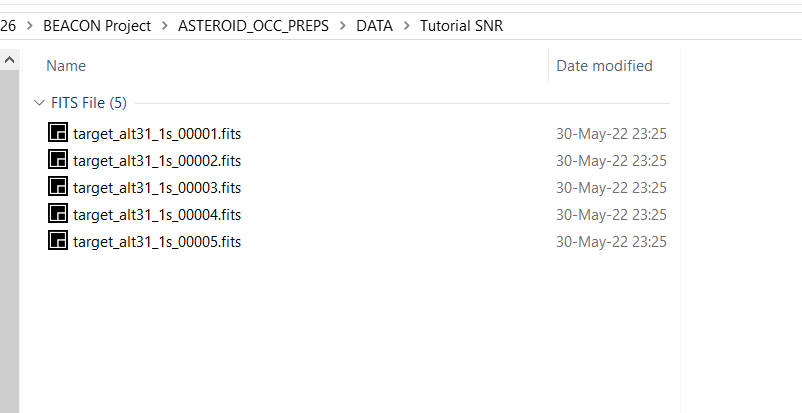
\includegraphics[width=0.6\linewidth]{snr_data_folder}
	\end{center}
	
	\item Buka \textsc{AIJ}, maka akan muncul tampilan berikut.
	\begin{center}
		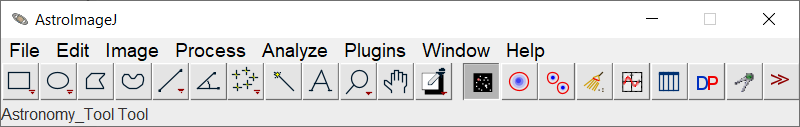
\includegraphics[width=0.6\linewidth]{snr_aij}
	\end{center}
	
	\item Pilih \textit{File > Import > Image Sequence}, maka akan muncul tampilan berikut. Centang 'Use virtual stack' untuk menghemat memori.
	
	\underline{Catatan:} tampilan frame berikut berada dalam mode \textit{invert}. Tekan logo dalam kotak merah untuk \textit{toggle}.
	\begin{center}
		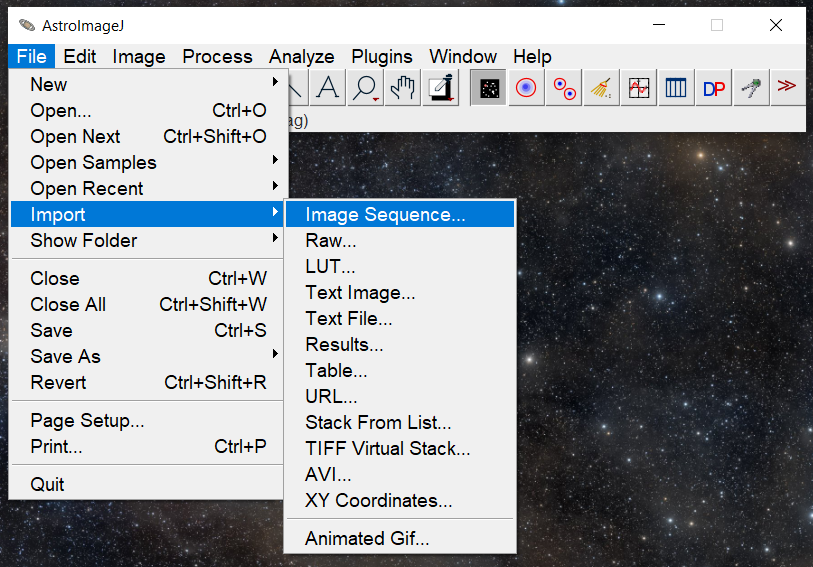
\includegraphics[width=0.6\linewidth]{snr_aij_import}
	\end{center}
	\begin{center}
		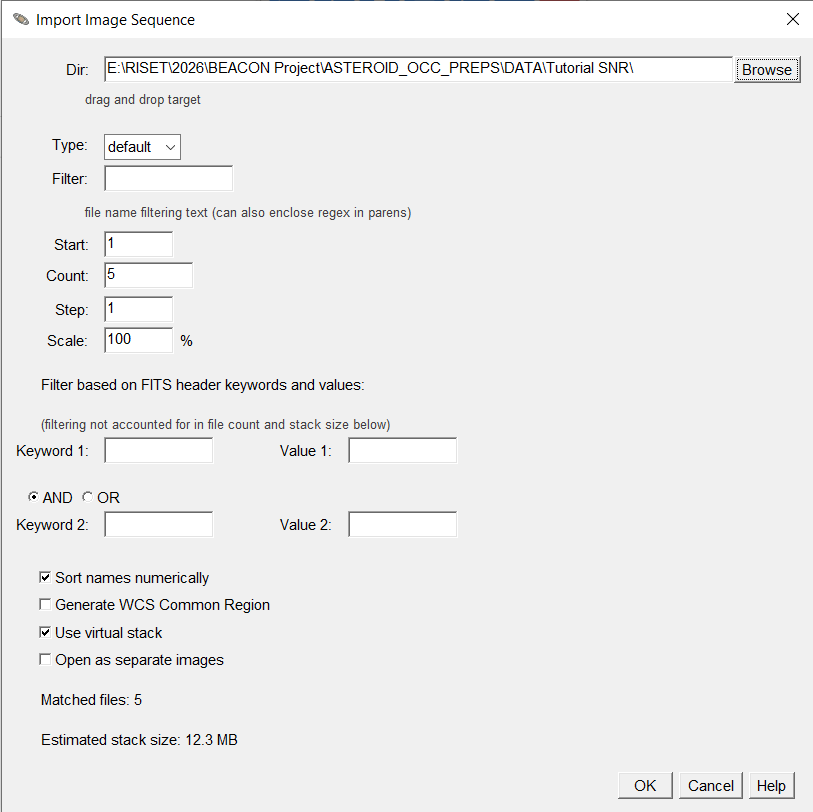
\includegraphics[width=0.6\linewidth]{snr_aij_virtualstack}
	\end{center}
	\begin{center}
		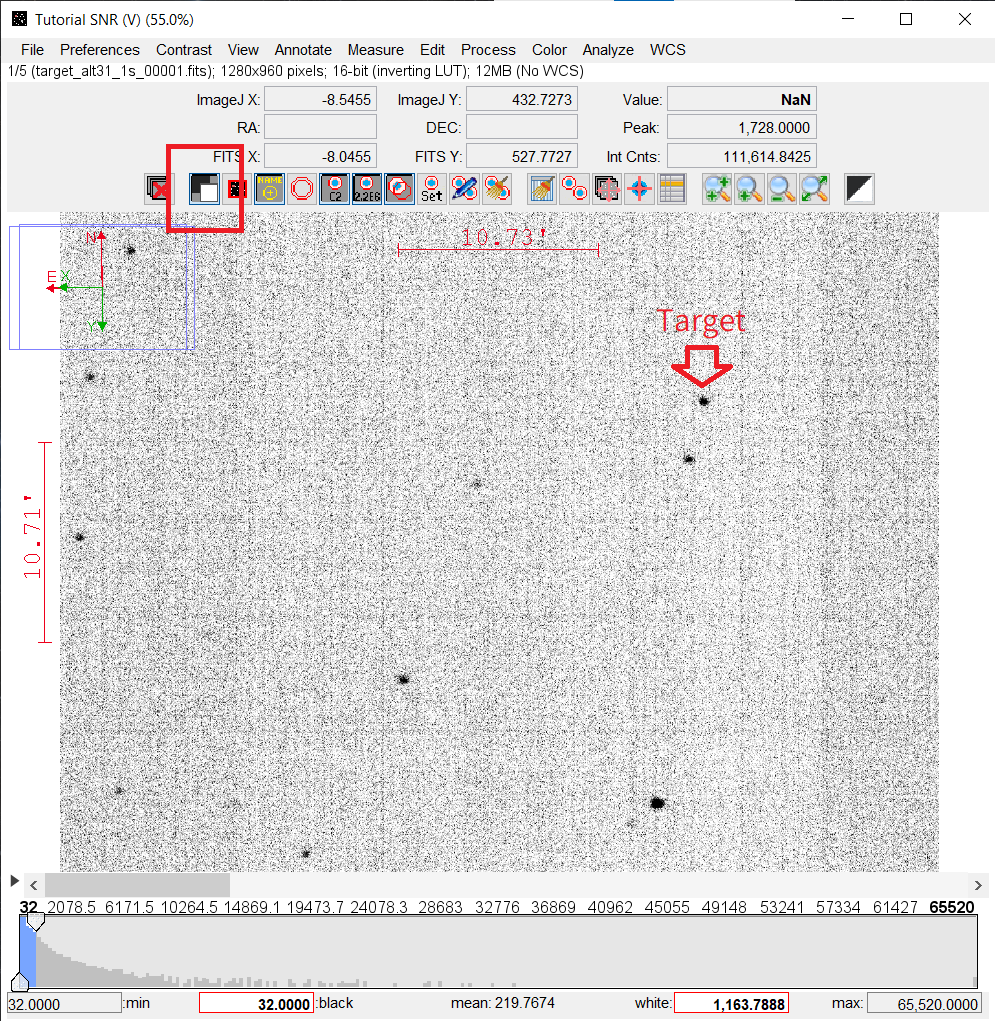
\includegraphics[width=0.6\linewidth]{snr_aij_toggle}
	\end{center}
	
	\item Tekan tombol alt + klik kiri pada bintang target, maka akan muncul profil \textit{seeing} bintang tersebut. Catat nilai HWHM (pada contoh ini HWHM = 3.39). Tekan tombol 'Save Aperture' dan tutup jendela tersebut. Jika ada salah menandai bintang, klik tombol 
\includegraphics[height=1em]{aij_clear} untuk menghapus aperture dan ulangi.
	\begin{center}
		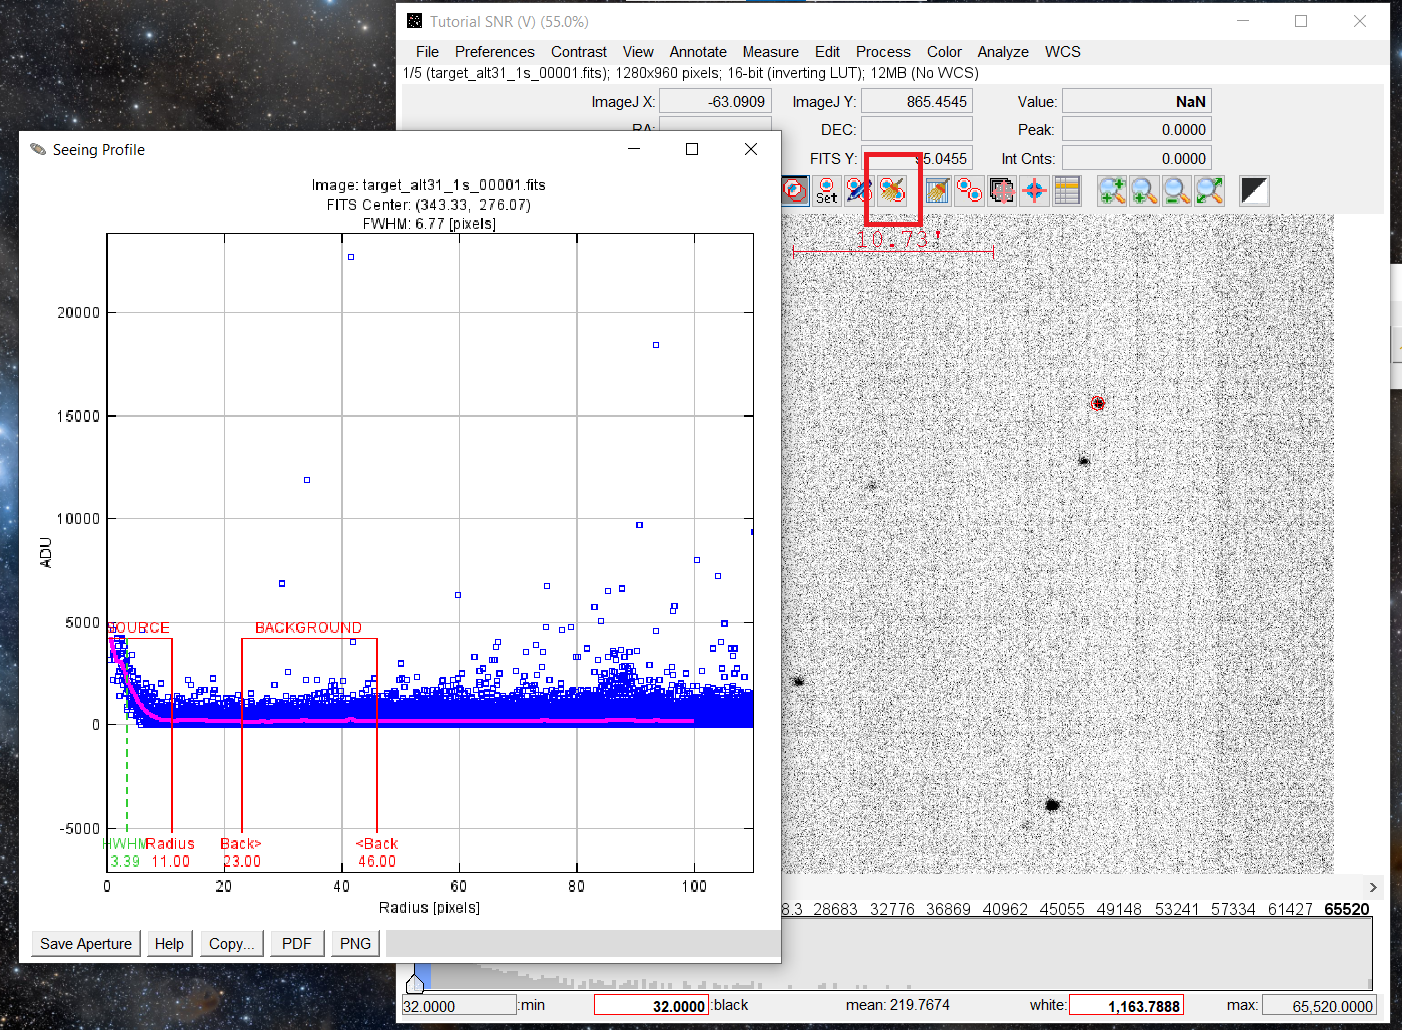
\includegraphics[width=0.6\linewidth]{snr_aij_seeing}
	\end{center}
	
	\item Klik tombol 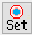
\includegraphics[height=1em]{aij_set} dan ubah beberapa parameter berikut.
	\begin{center}
		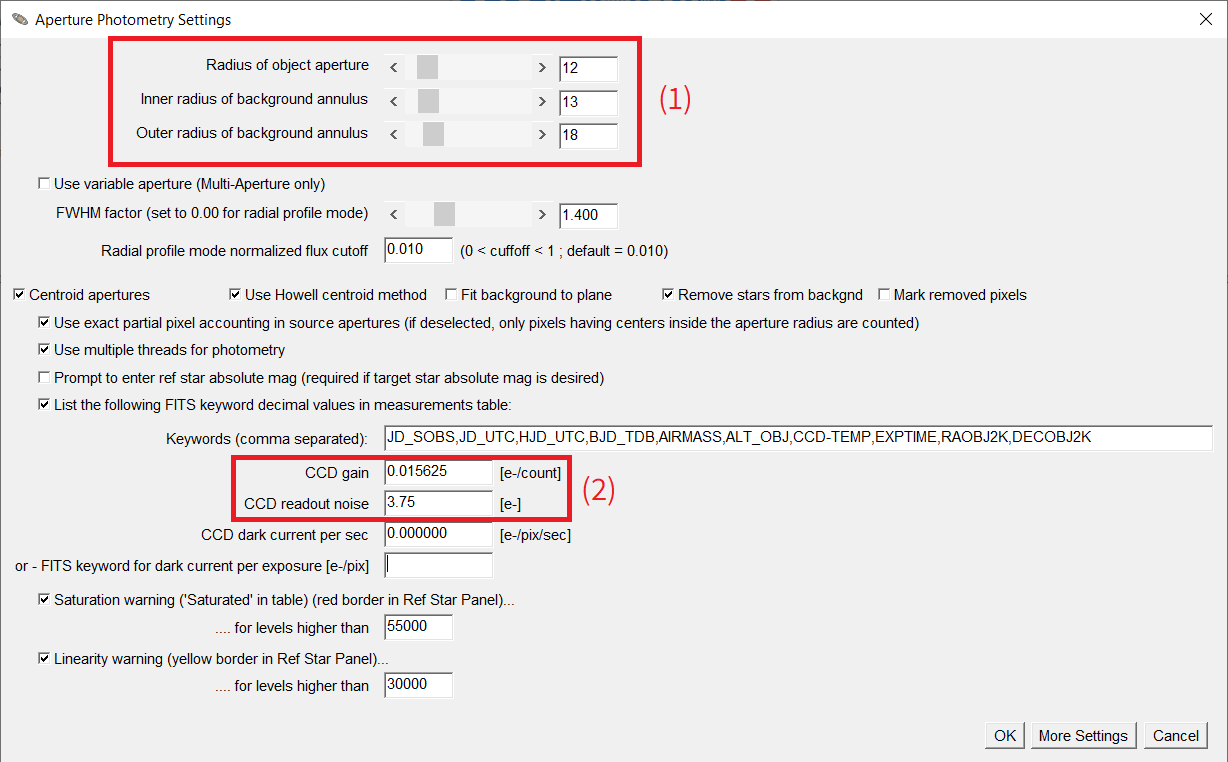
\includegraphics[width=0.6\linewidth]{snr_aij_aphot_settings}
	\end{center}
	\begin{enumerate}
		\item Untuk kotak (1):
		\begin{itemize}
			\item \textbf{Radius of object aperture}: $\sim 3-4$ kali HWHM.
			\item \textbf{Inner radius}: tambahkan $\sim 3$ poin dari \textbf{Radius of object aperture}.
			\item \textbf{Outer radius}: tambahkan $\sim 5$ poin dari \textbf{Inner radius}. Pastikan tidak ada bintang lain yang masuk dalam \textbf{Outer radius}.
			
			\underline{Catatan:} angka--angka di atas hanyalah \textit{guideline}. Cek dan sesuaikan dengan data yang dimiliki.
		\end{itemize}
		\item Untuk kotak (2):
		\begin{itemize}
			\item \textbf{CCD gain}: cek \textbf{CCD gain} untuk kamera anda (terlampir adalah beberapa contoh kurva gain. Sesuaikan dengan gain pada \textsc{SharCap}) dan bagi nilainya dengan 16 (karena mode 16--bit).
			
			\underline{Contoh:} untuk ZWO ASI120MM--S pada gain 75 (nilai di \textsc{SharpCap}), maka menurut kurva nilai gain--nya adalah $\sim 0.25$ e-/ADU. Maka nilai yang dimasukkan pada kotak (2) adalah 0.25/16 = 0.015625 e-/ADU.
			\begin{center}
				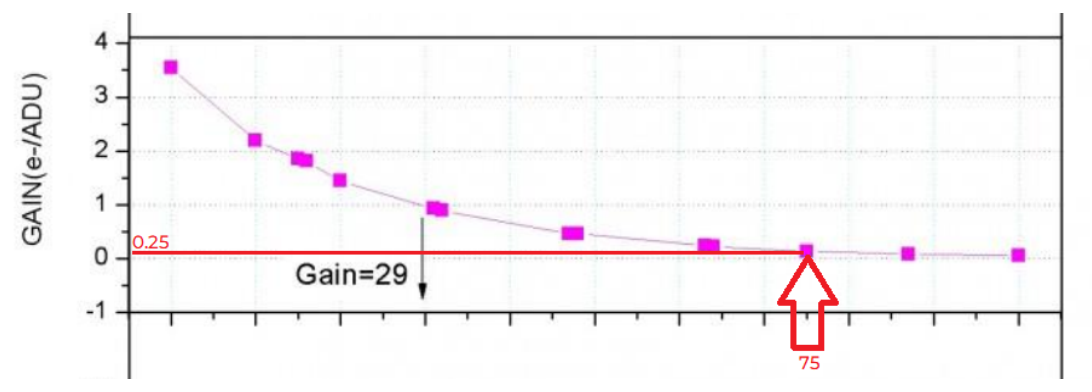
\includegraphics[width=0.7\linewidth]{snr_gain}
			\end{center}
			\item \textbf{CCD readout noise}: silakan merujuk kepada kurva terlampir untuk kamera yang digunakan. 
			
			\underline{Contoh:} pengamatan ini menggunakan gain 75, maka readout noise menurut kurva adalah $\sim 3.75$.
			\begin{center}
				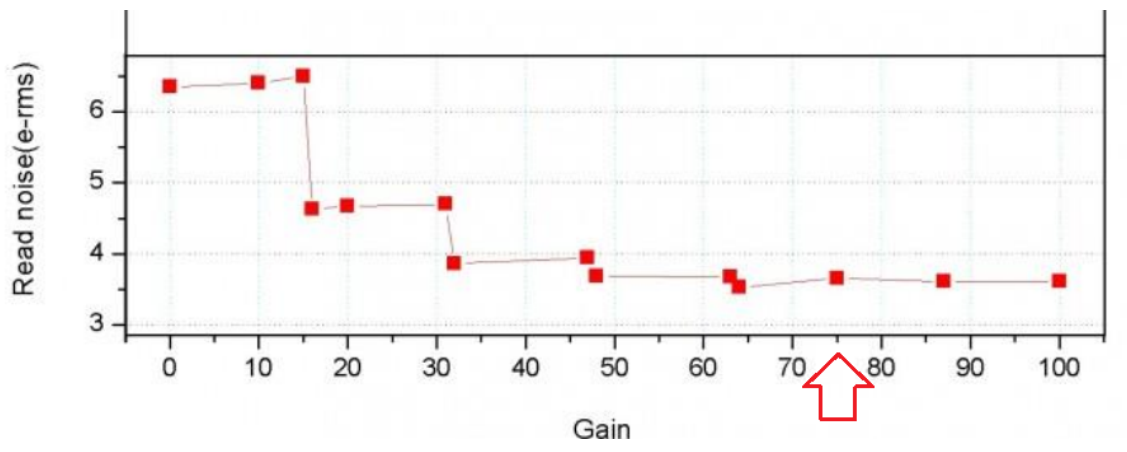
\includegraphics[width=0.7\linewidth]{snr_readout}
			\end{center}
		\end{itemize}
	\end{enumerate}
	Tekan OK untuk menutup jendela tersebut.
	
	\item Lakukan \textit{Star alignment}: klik \textit{Process > Align stack using WCS or apertures}.
	\begin{center}
		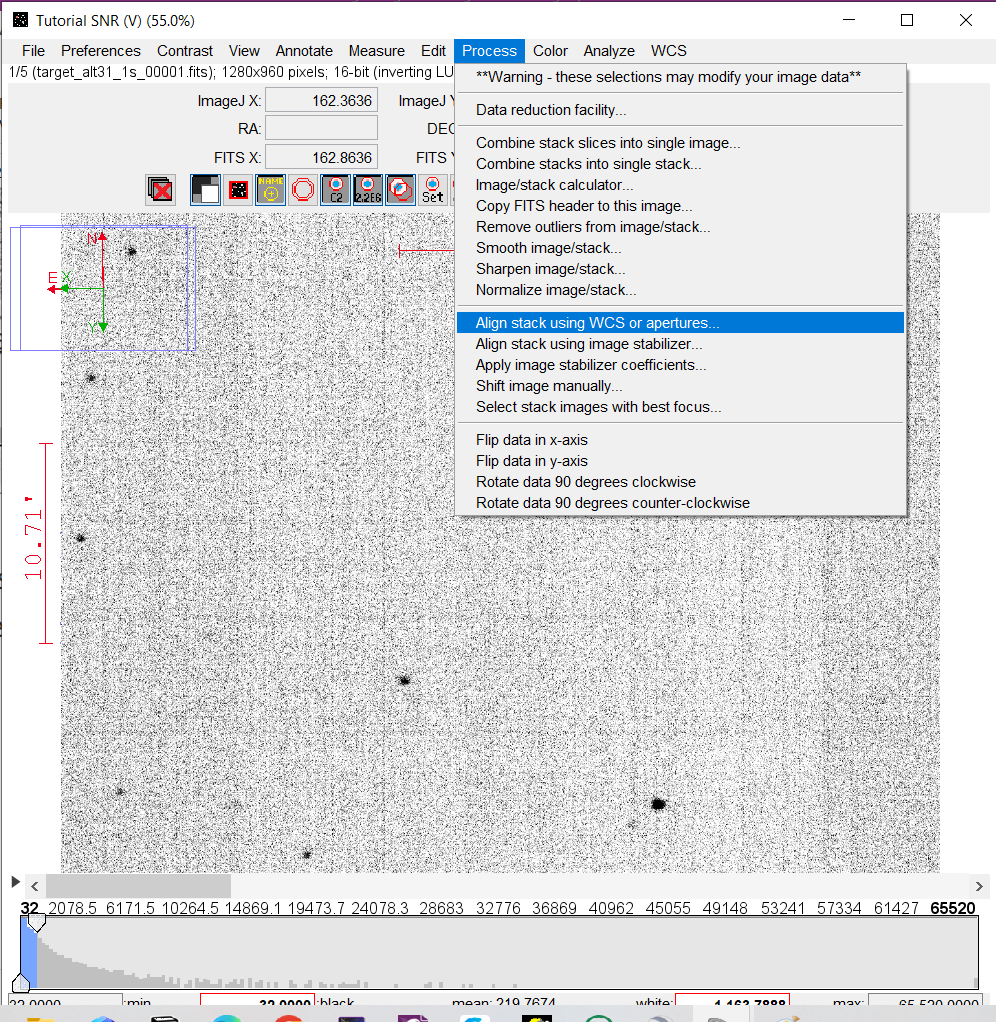
\includegraphics[width=0.6\linewidth]{snr_aij_align}
	\end{center}
	
	\item Pada jendela yang terbuka, pastikan \textit{First Slice} dan \textit{Last Slice} sudah sesuai dengan jumlah gambar (dalam contoh ini 5 gambar). Pastikan juga \textit{radius, inner radius, outer radius} sudah sesuai seperti poin sebelumnya. Sesuaikan \textit{setting} lain seperti pada gambar berikut. Tekan OK.
	\begin{center}
		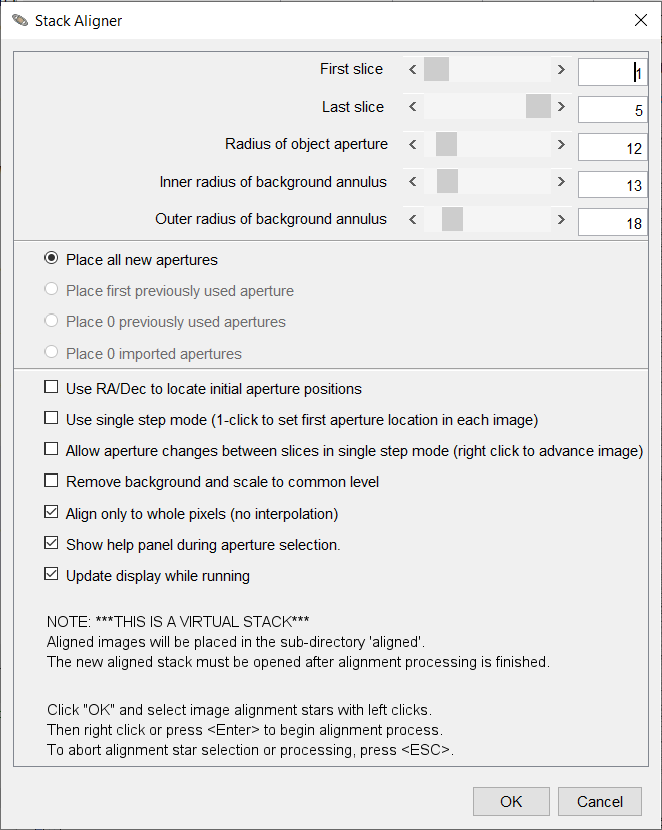
\includegraphics[width=0.6\linewidth]{snr_aij_stackaligner}
	\end{center}
	
	\item Arahkan kursor pada bintang target dan klik 1x, maka akan muncul aperture berwarna hijau. Klik juga bintang--bintang lain yang cukup terang, maka aperture merah akan muncul. Setelah selesai, tekan 'Enter'.
	\begin{center}
		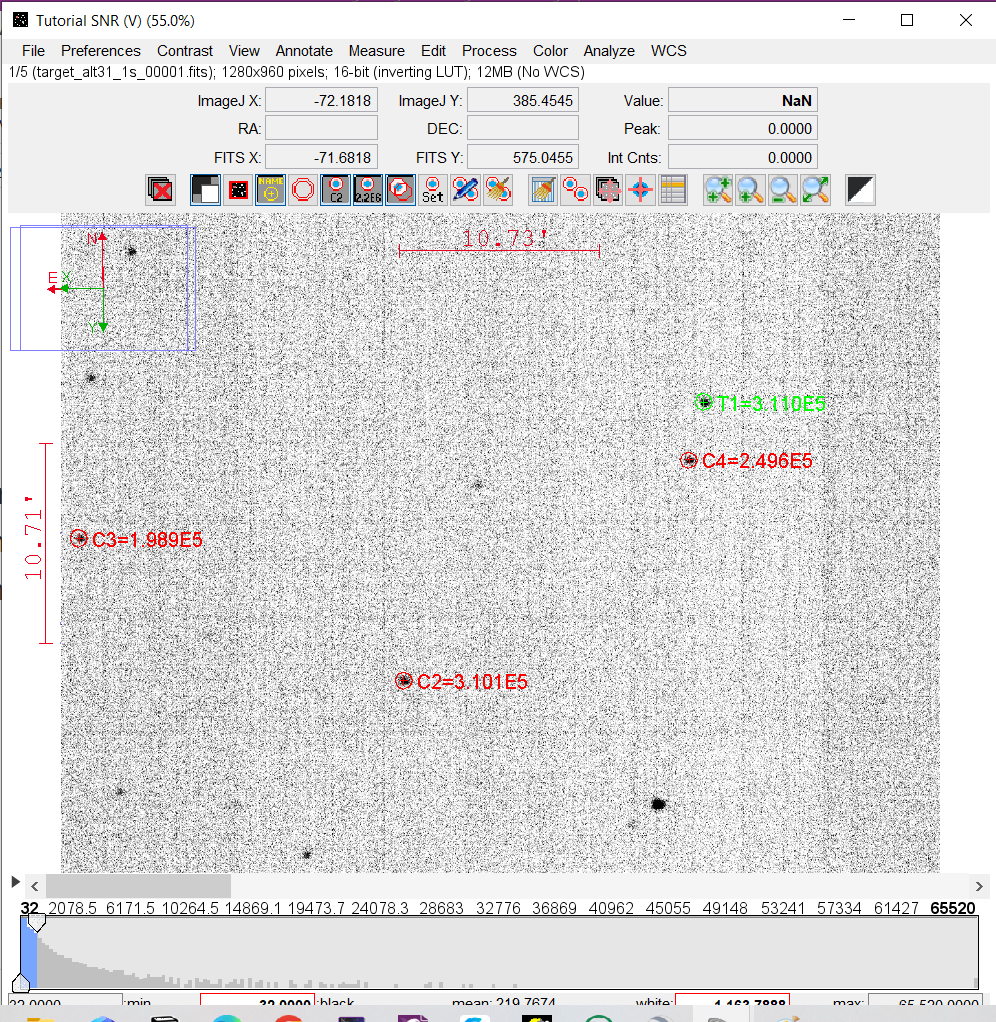
\includegraphics[width=0.6\linewidth]{snr_aij_select}
	\end{center}
	
	\item Setelah \textit{alignment} selesai, tekan OK/Yes dan tutup jendela citra. Direktori baru bernama 'aligned' akan muncul, berisi citra hasil \textit{alignment}.
	
	\item Lakukan \textit{File > Import > Image sequence} sekali lagi, namun arahkan ke direktori 'aligned' dan tekan OK. Maka akan muncul kembali jendela file citra. Cek dengan tombol panah kanan dan kiri untuk memastikan semua \textit{frame} telah \textit{aligned}.
	
	\item Tekan tombol 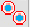
\includegraphics[height=1em]{aij_multiap} dan pastikan \textit{setting} kurang lebih seperti pada gambar berikut. \textit{First slice},
	\textit{Last Slice} dan parameter \textit{radius} akan berbeda untuk setiap set data. Tekan tombol 'Place Apertures'. 
	\begin{center}
		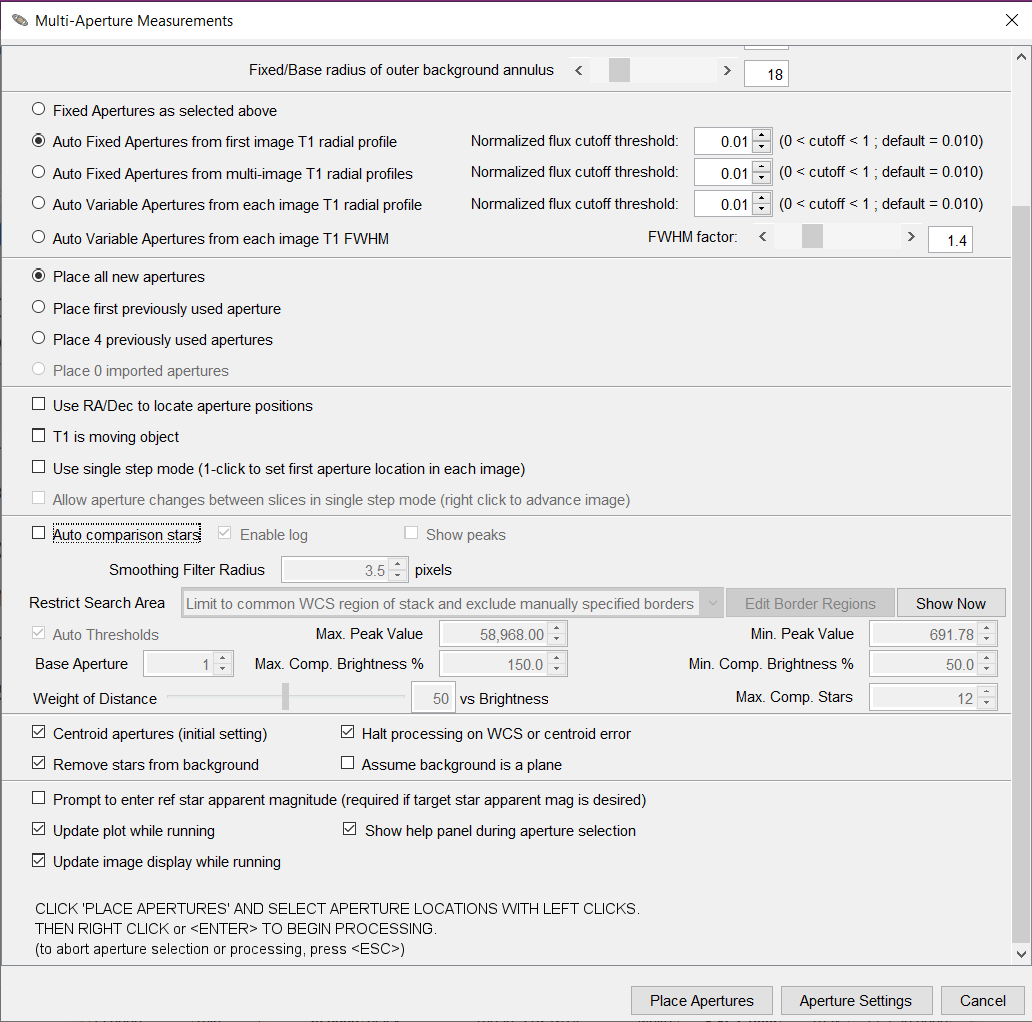
\includegraphics[width=0.6\linewidth]{snr_aij_multiap_measurement}
	\end{center}
	\begin{enumerate}
		\item Klik 1x pada bintang target (jangan sampai salah. Jika salah hapus dengan tombol 
\includegraphics[height=1em]{aij_clear}). klik juga pada bintang lain sebagai pembanding (optional, akan berguna jika anda ingin melakukan fotometri diferensial). Contoh pada dokumen ini menggunakan 1 bintang pembanding (aperture merah). Tekan 'Enter' untuk melakukan fotometri bukaan secara otomatis untuk semua frame. 
		\begin{center}
			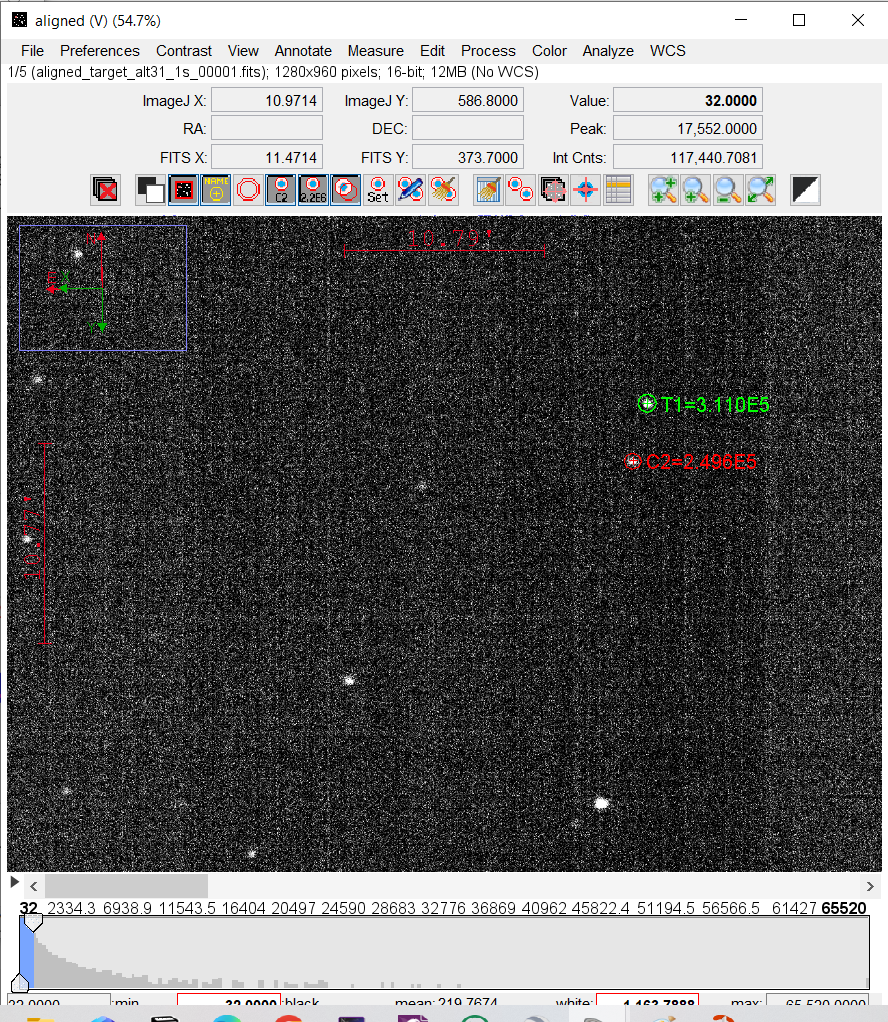
\includegraphics[width=0.7\linewidth]{snr_aij_aphot}
		\end{center}
		
		\item Akan muncul banyak jendela, abaikan untuk sementara. Saat proses selesai, cari jendela 'Measurements' (lihat gambar berikut) dan cari nilai SNR untuk target anda (kolom Source\_SNR\_T1 ). Ambil nilai rata--rata dari SNR ini.
		\begin{center}
			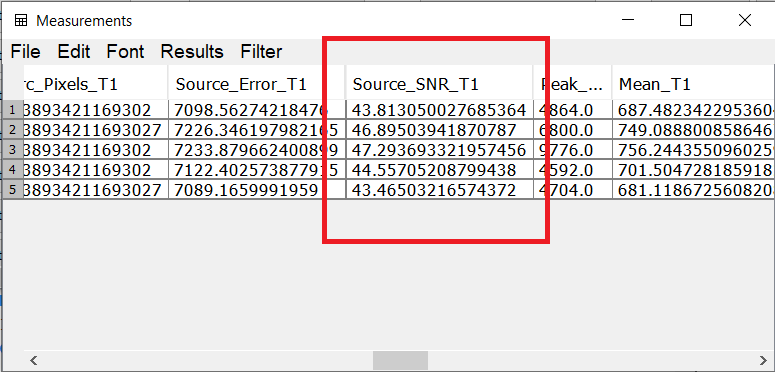
\includegraphics[width=0.7\linewidth]{snr_aij_snr}
		\end{center}
	\end{enumerate}
	\item Selamat! anda telah berhasil menghitung SNR data anda.
\end{enumerate}
\end{document}